\chapter{Sprint 02 – Gestion des prestataires}
\section*{Introduction}

Ce sprint est dédié à la mise en œuvre du module de gestion des prestataires (helpers) sur la plateforme Swift Helpers. Il vise à permettre aux prestataires de s’inscrire, compléter leur profil, consulter les services disponibles, exprimer leur intérêt, dialoguer avec les clients et suivre leur activité ainsi que leur rémunération.\\

La réalisation de ce sprint permet de renforcer l’autonomie des prestataires sur la plateforme en leur fournissant des interfaces intuitives et des fonctionnalités adaptées à leur rôle.\\

Les éléments livrés dans ce sprint incluent :
\begin{itemize}
  \item L’implémentation du processus d’inscription et de complétion du profil helper ;
  \item L’intégration de l’interface de consultation des ordres disponibles avec la possibilité d’exprimer un intérêt ;
  \item La mise en place de la messagerie entre prestataire et client ;
  \item La visualisation du calendrier des missions planifiées ;
  \item Le tableau de bord de suivi des prestations et des paiements ;
  \item La consultation des factures.
\end{itemize}

L’ensemble de ces développements est conforme aux spécifications fonctionnelles définies précédemment et respecte la logique modulaire Angular intégrée à une architecture backend Django.
\section*{Sprint 02 Backlog}

\begin{center}
\begin{tabular}{|c|p{4.2cm}|c|p{4.5cm}|c|c|}
\hline
\textbf{ID US} & \textbf{User Story} & \textbf{ID Task} & \textbf{Task} & \textbf{Estimation} & \textbf{Responsable} \\
\hline
2.1 & En tant que prestataire, je veux créer et gérer mon compte & 2.1.1 & Implémenter le formulaire d’inscription helper & 3h & Aziz \\
\cline{3-6}
& & 2.1.2 & Implémenter le formulaire de complétion de profil & 3h & Aziz \\
\cline{3-6}
& & 2.1.3 & Tester la logique de sauvegarde des données & 2h & Aziz \\
\hline
2.2 & En tant que prestataire, je veux consulter les ordres disponibles et exprimer mon intérêt & 2.2.1 & Implémenter l’interface des ordres & 2h & Aziz \\
\cline{3-6}
& & 2.2.2 & Implémenter le bouton “exprimer l’intérêt” & 2h & Aziz \\
\cline{3-6}
& & 2.2.3 & Implémenter la messagerie avec le client & 3h & Aziz \\
\hline
2.3 & En tant que prestataire, je veux suivre mon travail et mes factures & 2.3.1 & Implémenter l’agenda des prestations & 2h & Aziz \\
\cline{3-6}
& & 2.3.2 & Implémenter l’interface de suivi des revenus & 2h & Aziz \\
\cline{3-6}
& & 2.3.3 & Implémenter la visualisation des factures & 2h & Aziz \\
\hline
\end{tabular}
\end{center}

\section*{Diagramme de cas d’utilisation raffiné – Prestataire}

\begin{figure}[H]
\centering
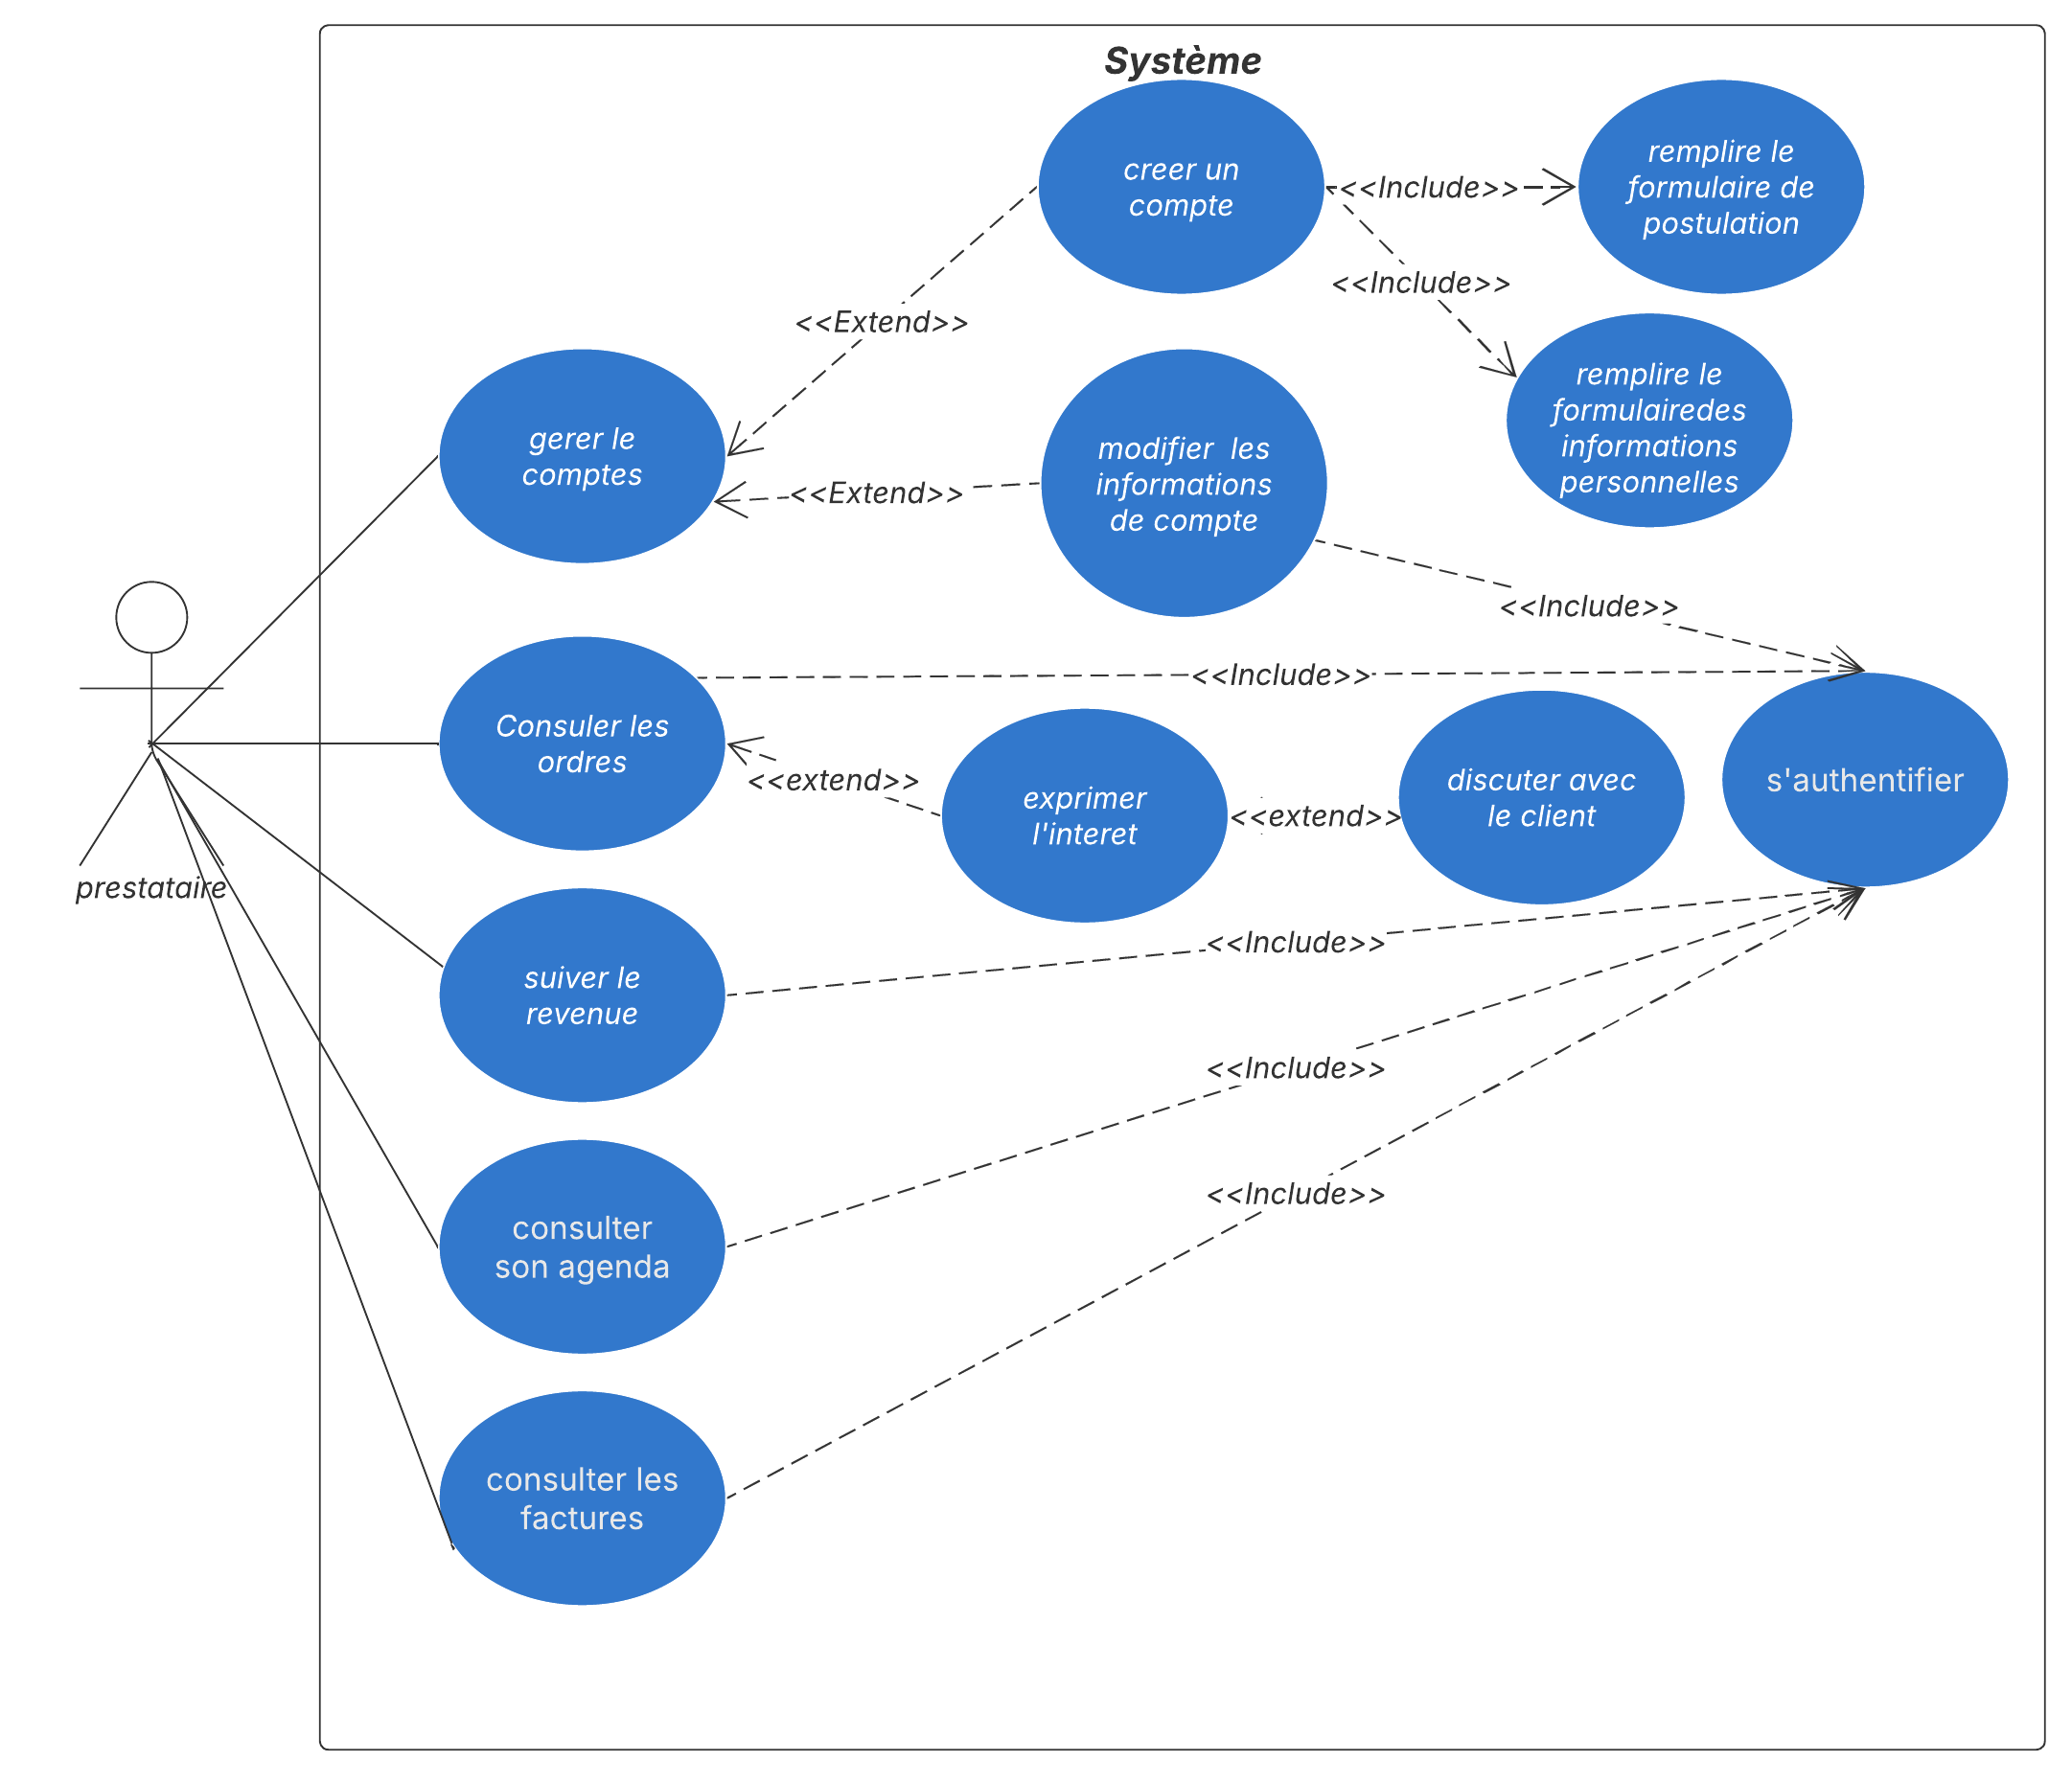
\includegraphics[width=0.8\linewidth]{figures/Diagramme de cas d'utilisation (1).png}
\caption{Diagramme de cas d’utilisation raffiné pour le rôle Prestataire}
\end{figure}

\textit{Ce diagramme met en évidence les différentes interactions d’un prestataire avec le système, incluant la gestion de son compte, la consultation des ordres, l’expression d’intérêt, la messagerie avec le client, le suivi de son agenda, de ses revenus et de ses factures.}

\section*{Interfaces utilisateur Angular – Prestataire}

\begin{figure}[H]
\centering
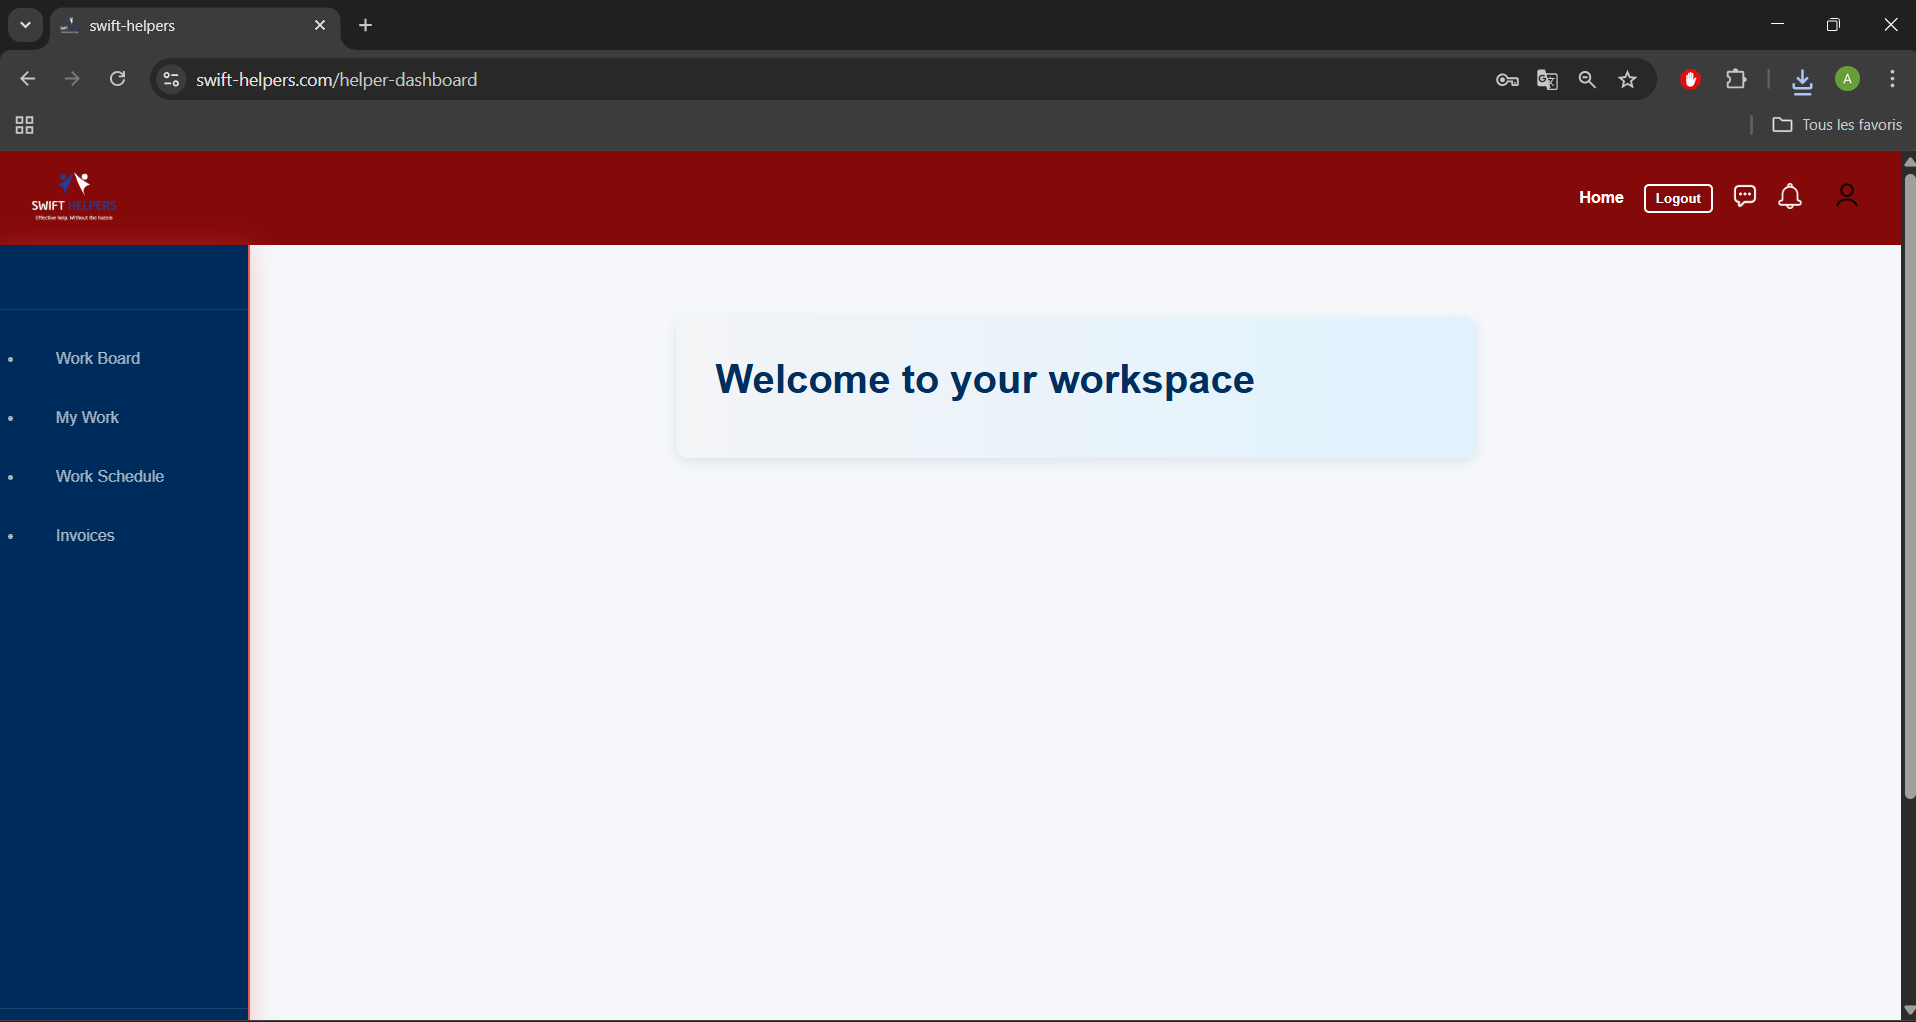
\includegraphics[width=0.85\linewidth]{figures/helper dashboard.png}
\caption{Dashboard du prestataire}
\end{figure}
\textit{Interface d’accueil personnalisée pour le prestataire avec navigation latérale vers les modules clés.}\\
Cette interface est le point d’entrée principal du prestataire. Elle lui donne une vue d’ensemble et un accès rapide aux principales sections telles que les ordres, les factures ou le calendrier de travail.

\begin{figure}[H]
\centering
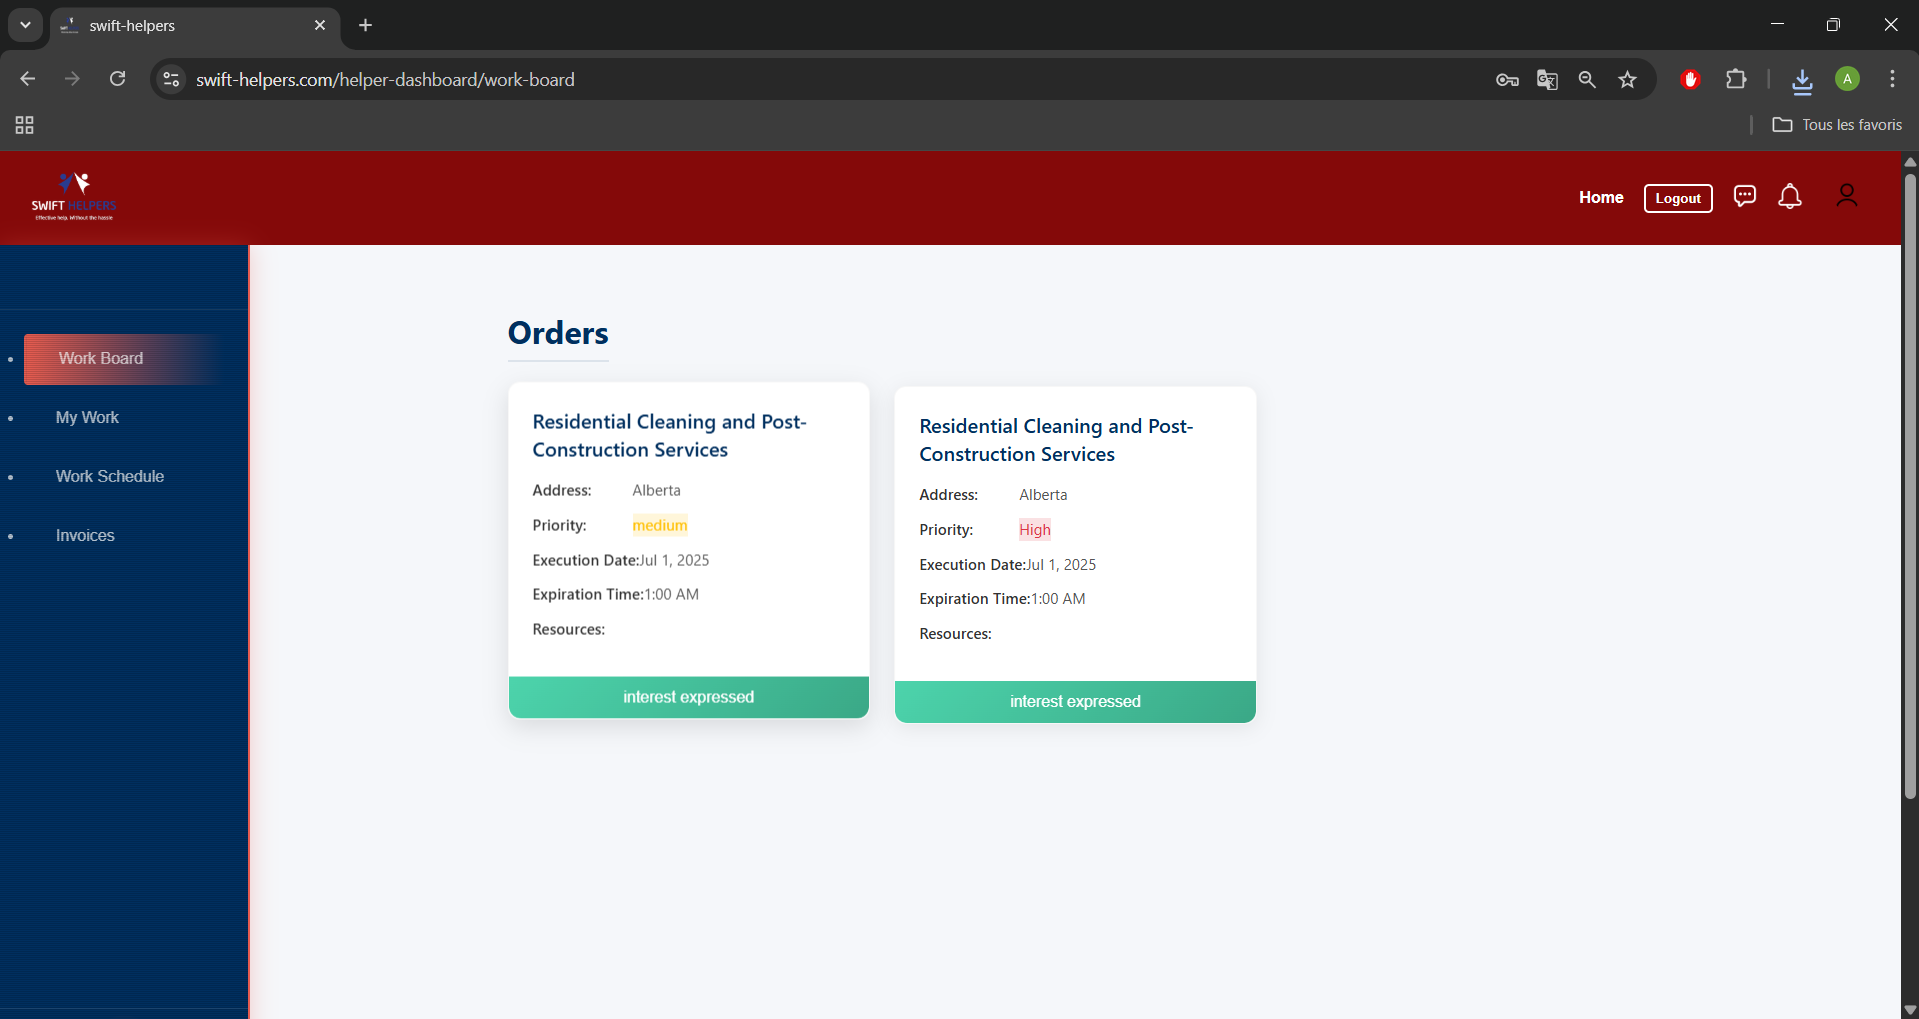
\includegraphics[width=0.85\linewidth]{figures/orders.png}
\caption{Liste des ordres disponibles}
\end{figure}
\textit{Vue des services disponibles avec priorités et détails. Le prestataire peut exprimer son intérêt.}\\
Chaque carte présente les informations essentielles : adresse, date d’exécution, priorité et expiration. Le prestataire peut cliquer sur un bouton pour signaler son intérêt, ce qui déclenche le processus de mise en relation.

\begin{figure}[H]
\centering
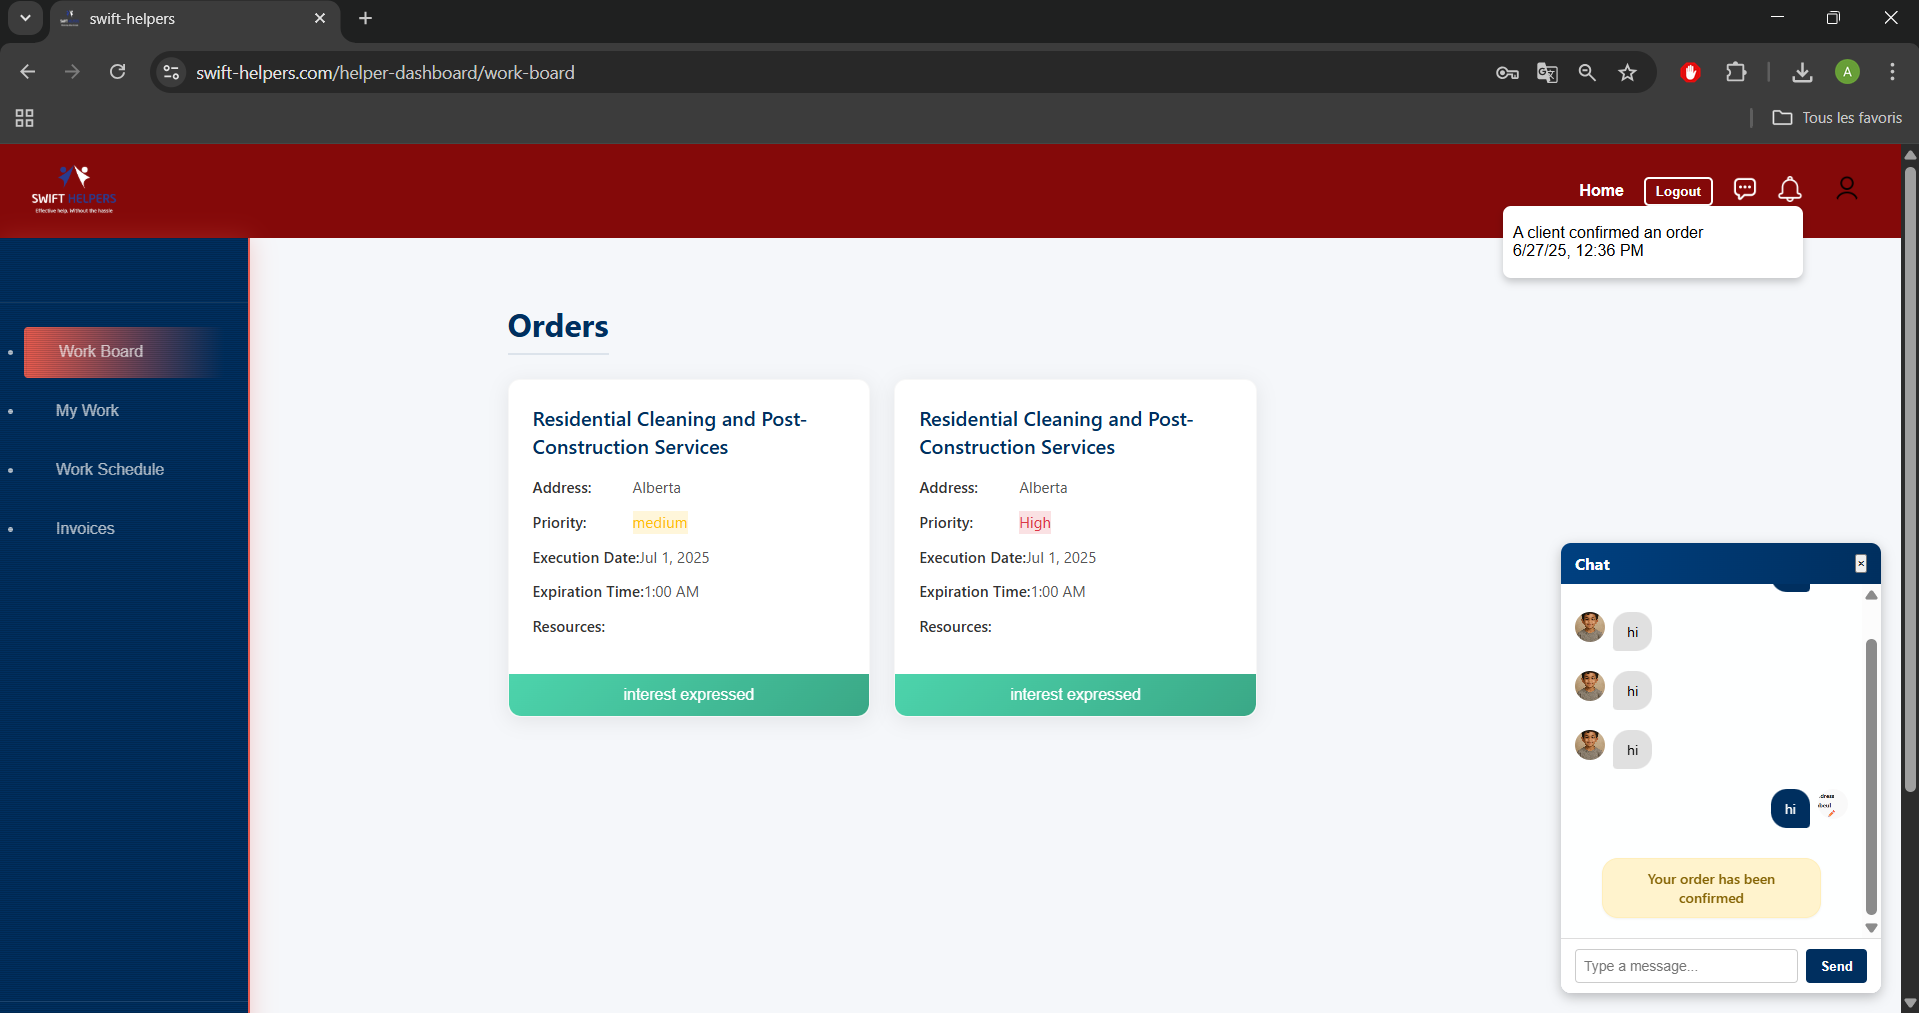
\includegraphics[width=0.85\linewidth]{figures/discussion.png}
\caption{Messagerie prestataire-client}
\end{figure}
\textit{Système de messagerie intégré pour la communication avec le client.}\\
Cette messagerie permet d’échanger en temps réel sur les détails de la mission. Elle favorise une communication fluide avant et après l’exécution du service, augmentant ainsi la qualité de l’interaction.

\begin{figure}[H]
\centering
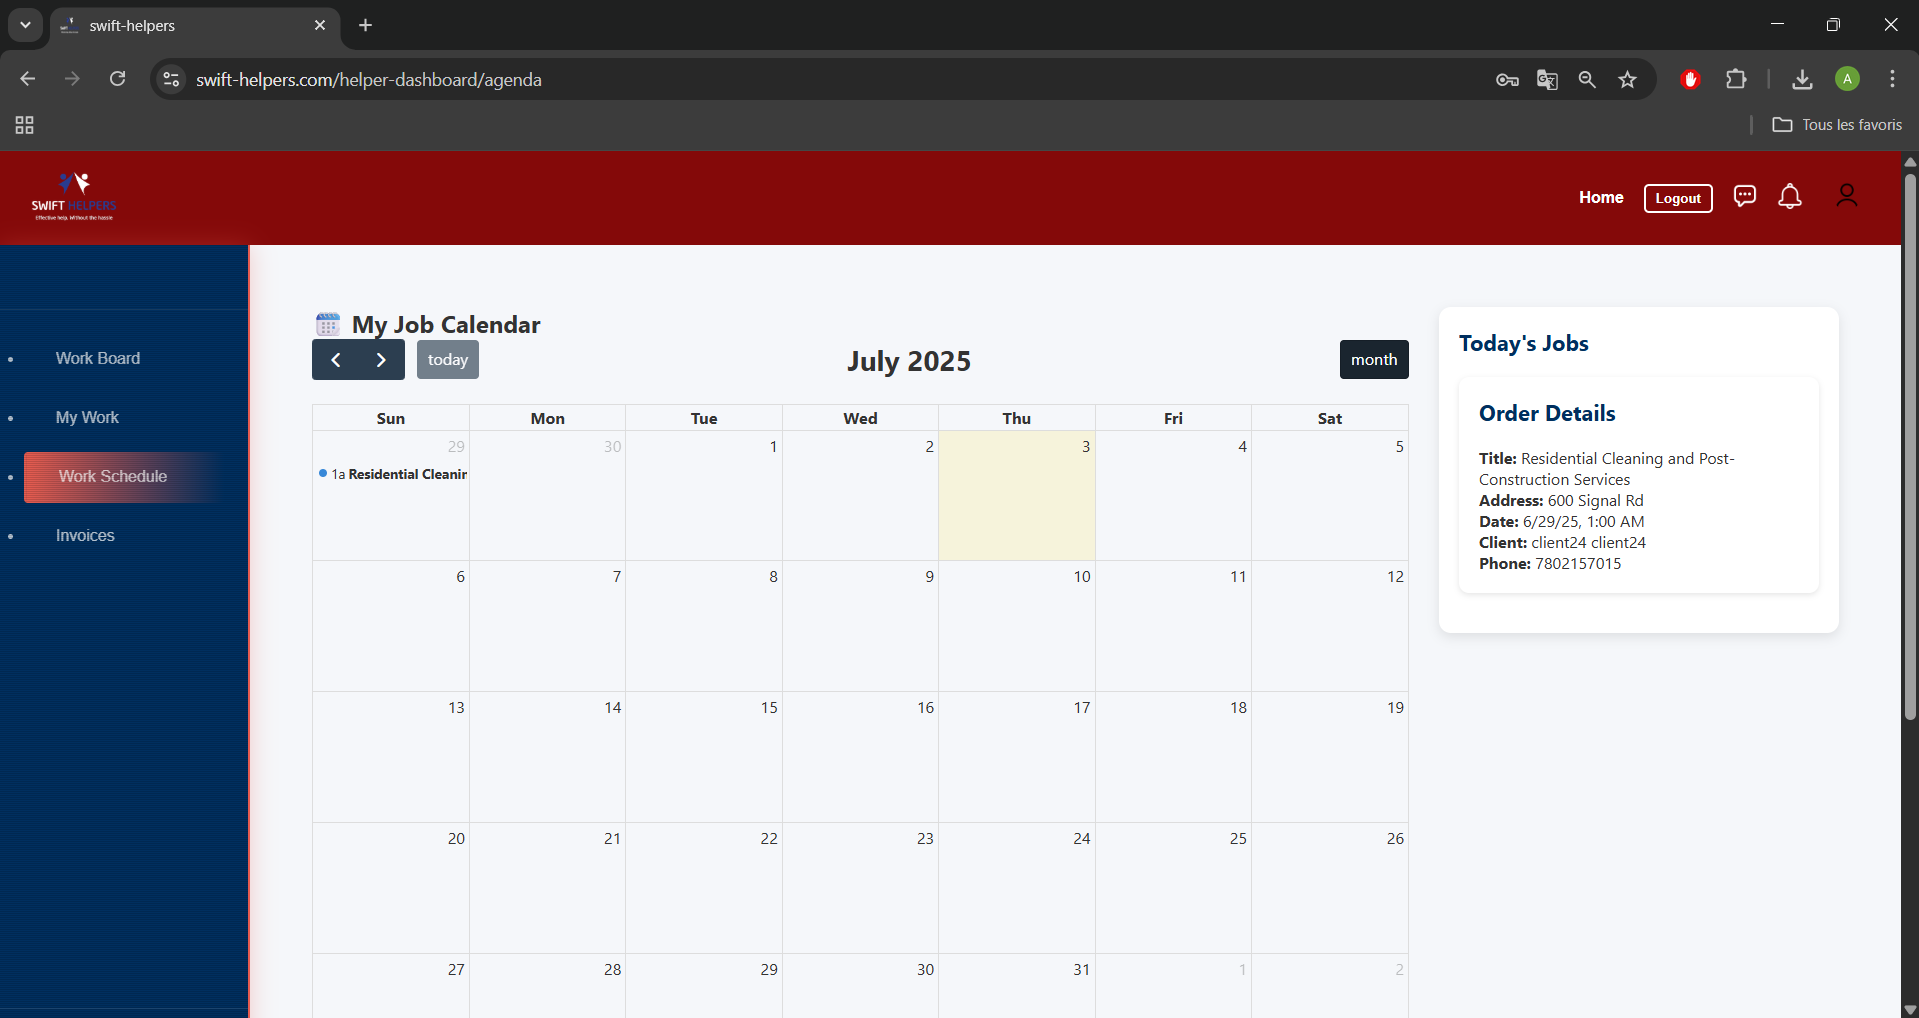
\includegraphics[width=0.85\linewidth]{figures/schedules.png}
\caption{Suivi de l’agenda}
\end{figure}
\textit{Calendrier interactif affichant les missions confirmées avec détails.}\\
Le prestataire peut visualiser les missions confirmées par date. Une carte d'information présente le titre, l'adresse, le client concerné et l’heure d’exécution. Cela permet une meilleure planification de ses activités.

\begin{figure}[H]
\centering
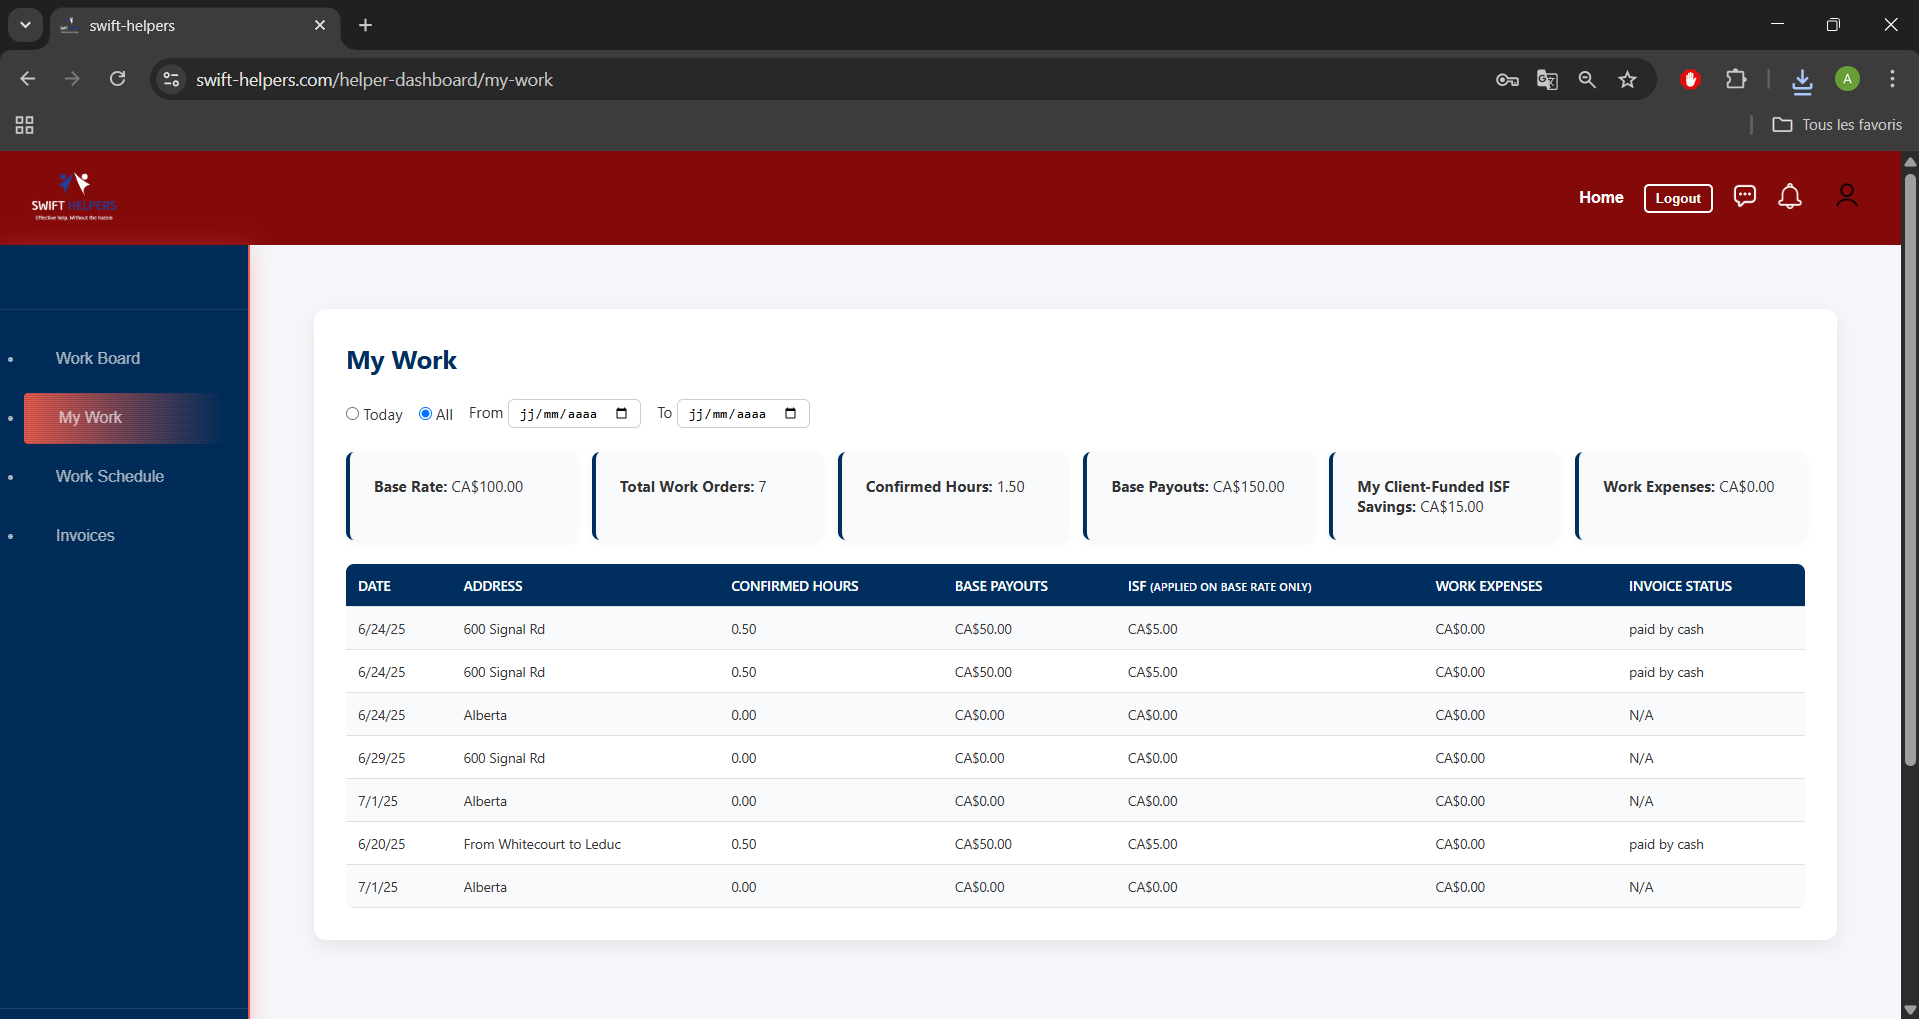
\includegraphics[width=0.85\linewidth]{figures/work.png}
\caption{Suivi des missions et revenus}
\end{figure}
\textit{Interface synthétique du travail effectué, heures confirmées, rémunérations et statut de paiement.}\\
Cette vue agrège les données importantes liées aux prestations : heures validées, paiements générés, économies ISF, et dépenses. Elle sert de tableau de bord de performance pour le prestataire.

\begin{figure}[H]
\centering
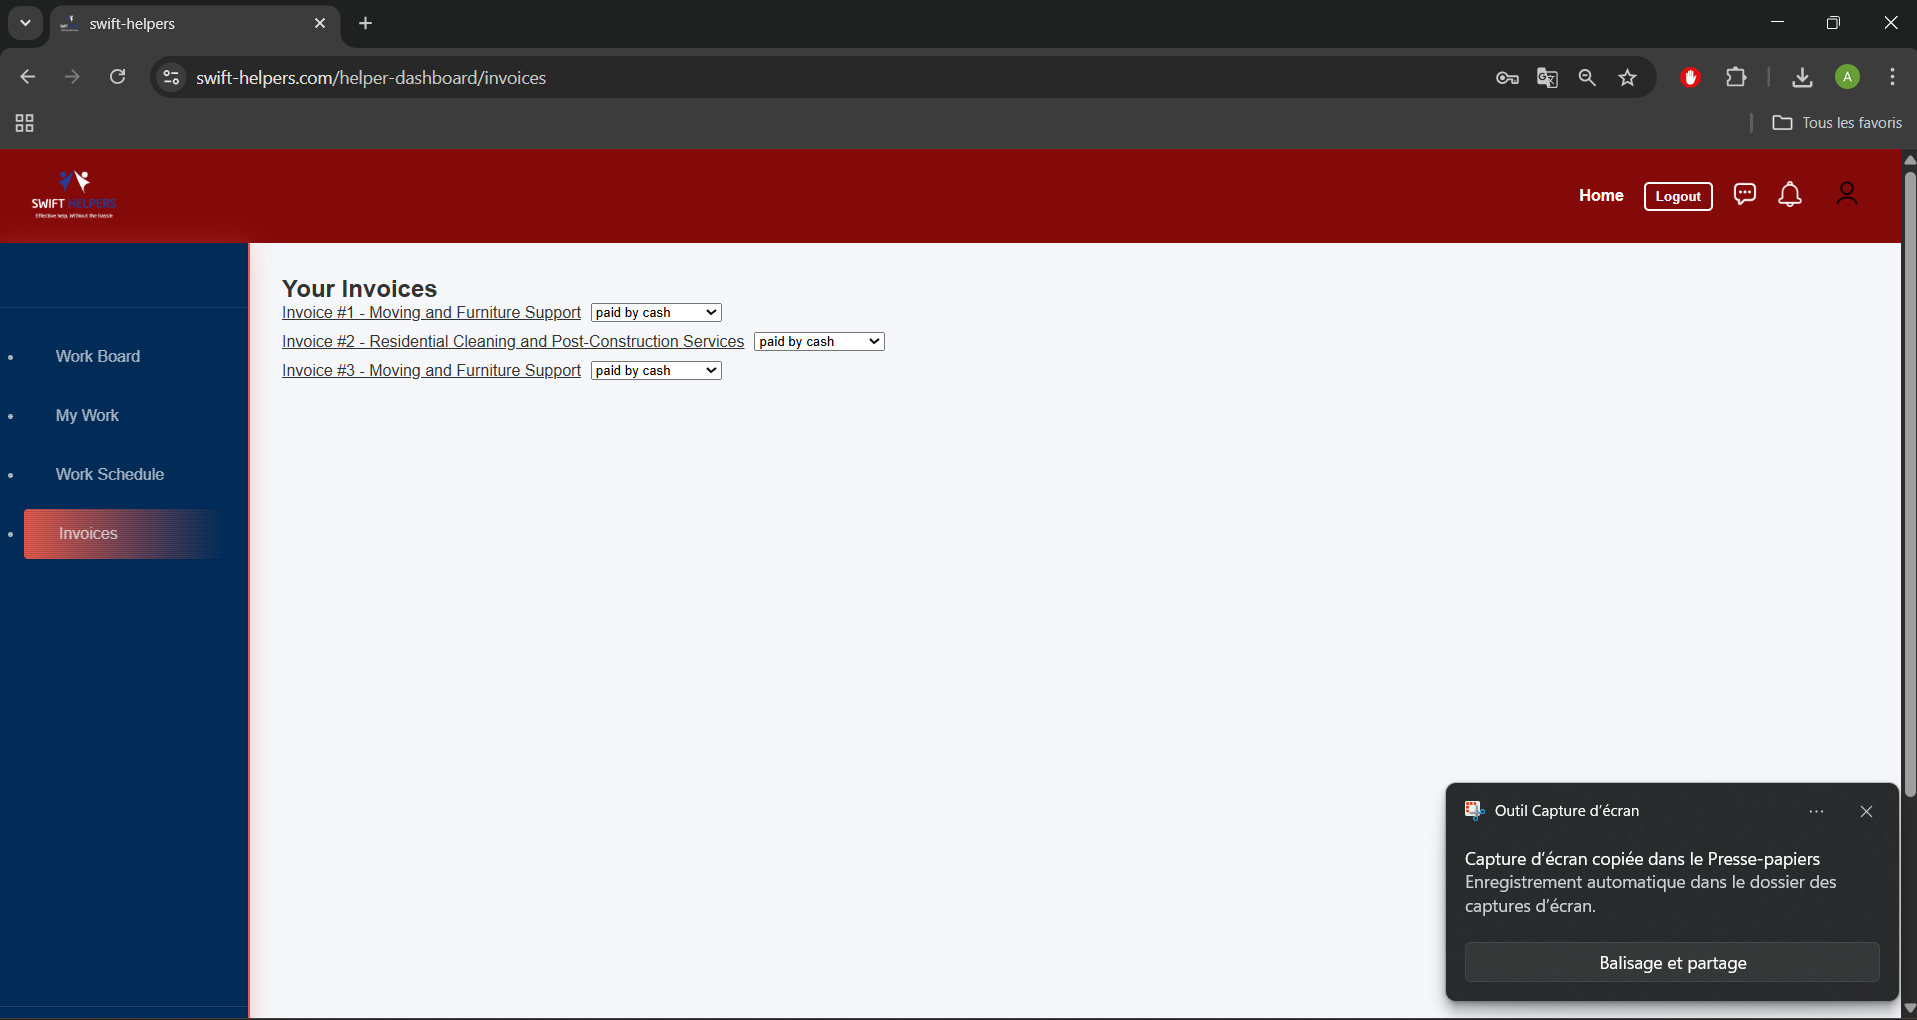
\includegraphics[width=0.85\linewidth]{figures/invoices.png}
\caption{Consultation des factures}
\end{figure}
\textit{Historique des factures avec option de tri par service et statut de paiement.}\\
L’interface permet de filtrer les factures générées automatiquement selon le type de service ou le mode de paiement (ex. cash). Elle offre un historique clair et facilite le suivi administratif.
\section*{Aperçu sur le code – Prestataire}

\begin{figure}[H]
\centering
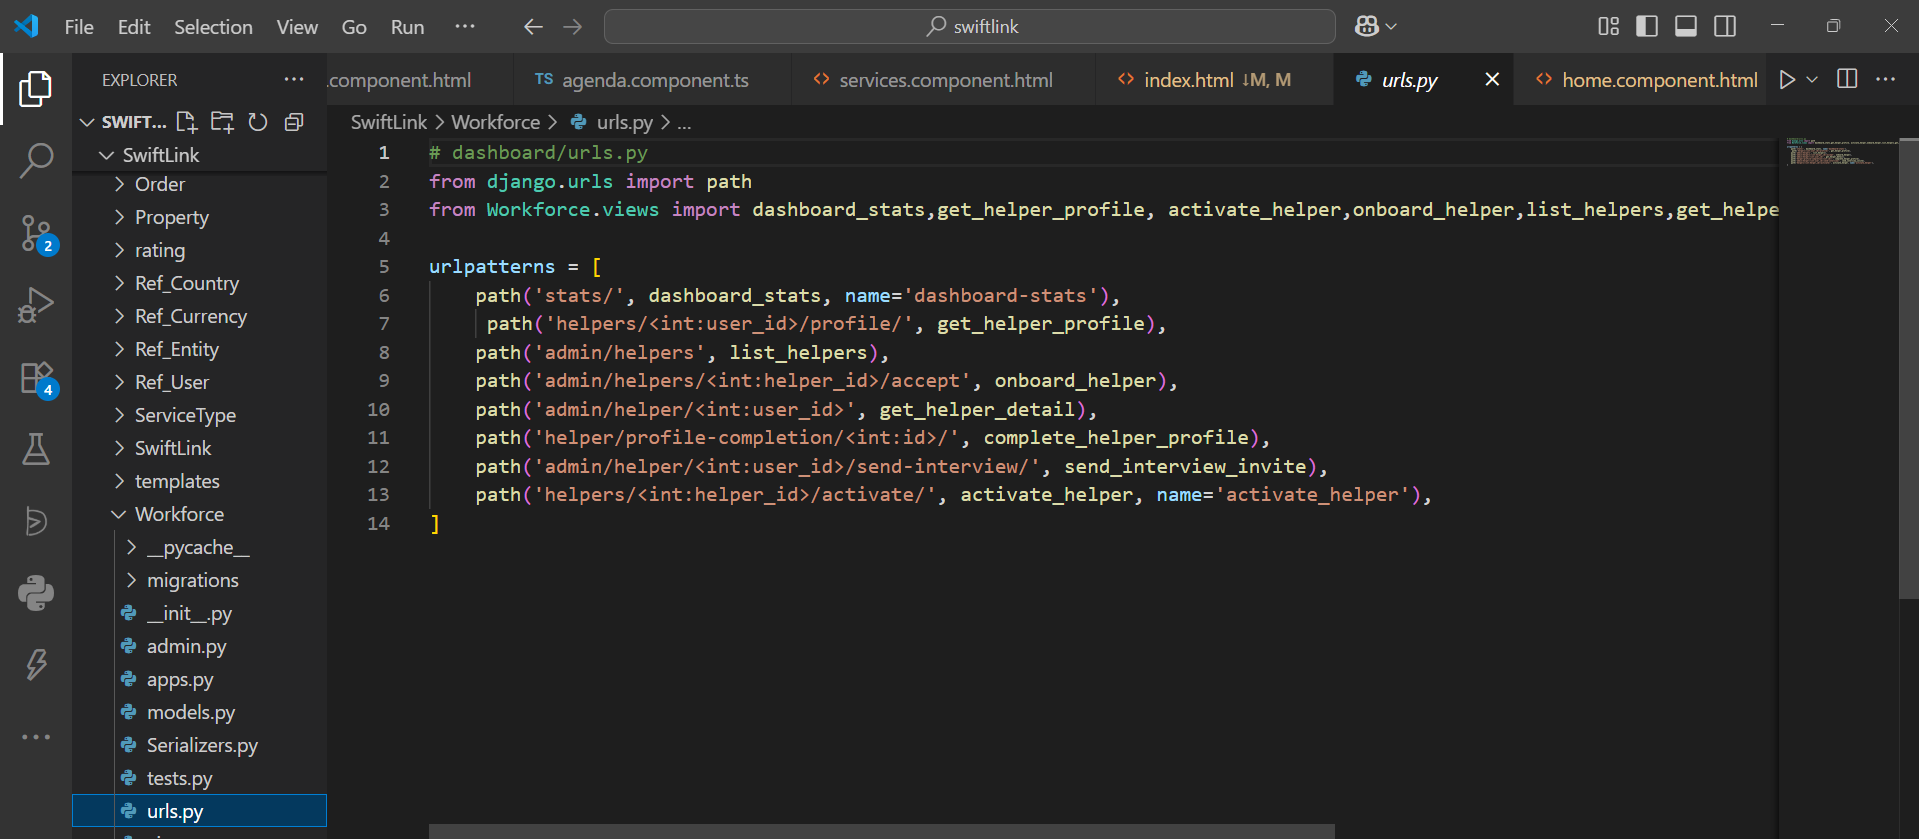
\includegraphics[width=0.85\linewidth]{figures/helper urls.png}
\caption{Fichier \texttt{urls.py} – Définition des routes pour les helpers}
\end{figure}
\textit{Ce fichier \texttt{urls.py} dans le module \texttt{Workforce} déclare les routes backend pour la gestion des prestataires. On y retrouve les chemins pour accéder aux statistiques, gérer les profils, accepter ou activer un helper, et envoyer une invitation à l’entretien. Chaque route est liée à une vue correspondante côté Django.}

\vspace{0.5cm}

\begin{figure}[H]
\centering
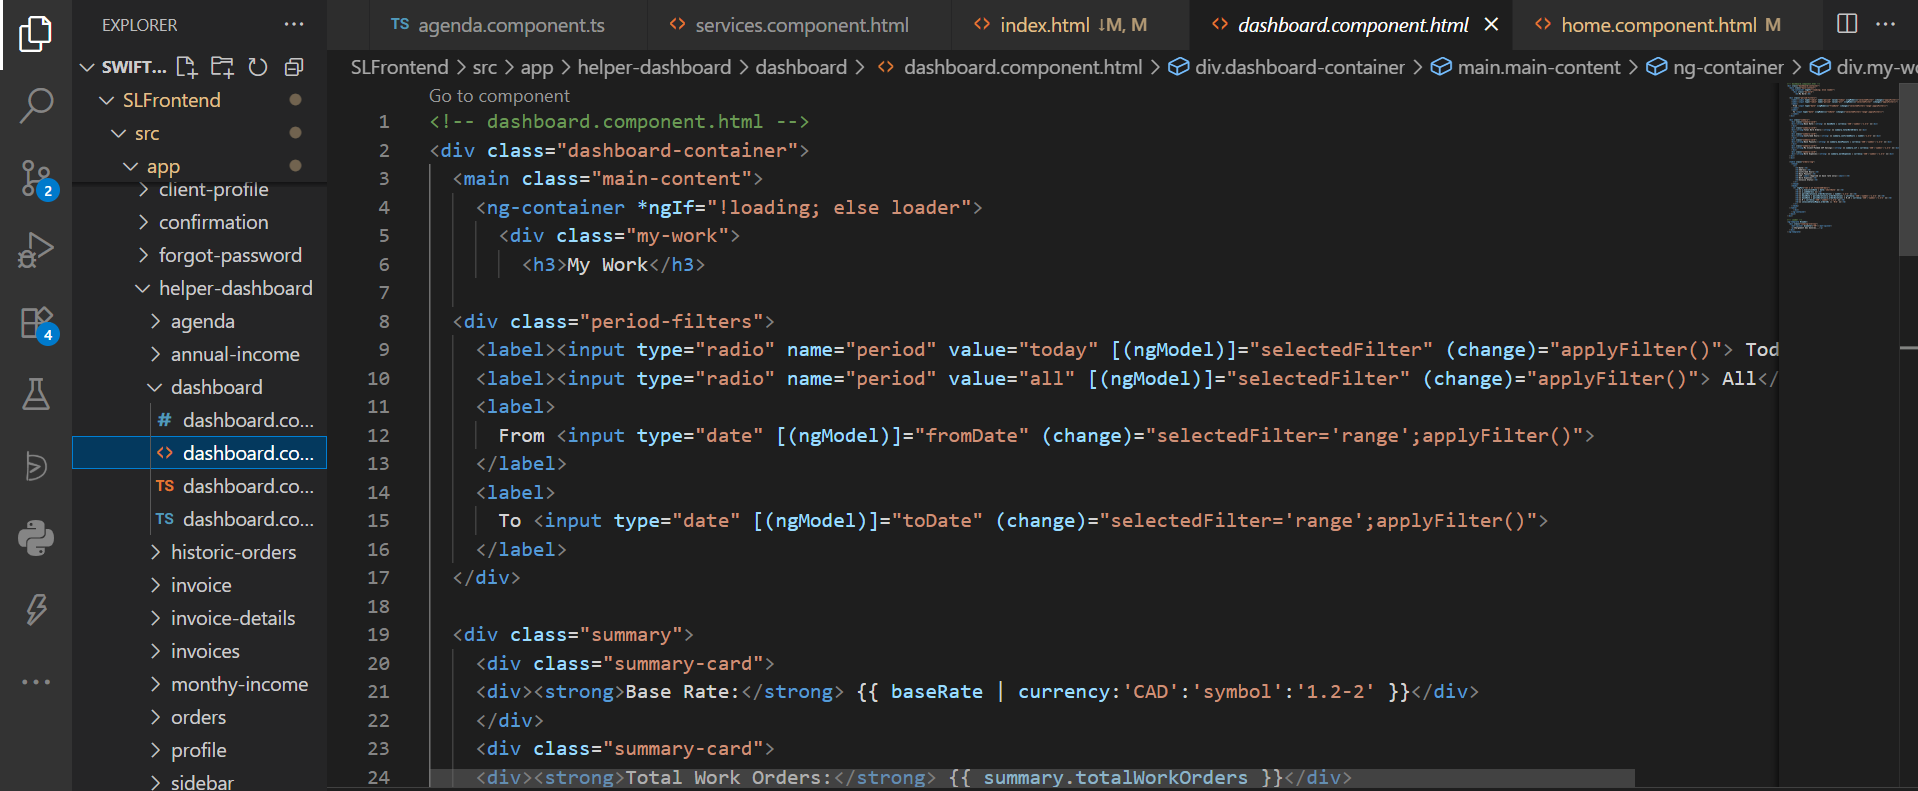
\includegraphics[width=0.85\linewidth]{figures/helper dash.png}
\caption{Fichier \texttt{dashboard.component.html} – Affichage du tableau de bord}
\end{figure}
\textit{Le fichier \texttt{dashboard.component.html} construit l’interface du tableau de bord pour le prestataire. Il affiche les informations de synthèse comme le taux horaire, le nombre total de missions et les revenus, avec des filtres de période via des boutons radio ou des champs de date. Ce composant Angular permet une vue analytique du travail effectué.}

\section*{Conclusion}

Ce sprint a permis de concrétiser un pan essentiel du fonctionnement de la plateforme Swift Helpers : l’autonomie et l’interaction efficace des prestataires avec le système. Grâce aux interfaces développées et à l’intégration fluide entre les composants frontend et backend, les helpers disposent désormais d’un environnement complet pour gérer leur activité.

L’implémentation des différentes fonctionnalités – de l’inscription à la consultation des missions, en passant par la messagerie et le suivi de la facturation – constitue un socle opérationnel solide sur lequel pourront s’appuyer les modules métier futurs.

La modularité du code Angular et la robustesse des API Django garantissent par ailleurs une bonne évolutivité du système. Ce sprint a ainsi répondu pleinement aux objectifs fixés et constitue une étape clé dans l’extension fonctionnelle de la plateforme.

